\documentclass[11pt]{article}

% load some asm stuff -
\usepackage{amssymb}
\usepackage{amsmath}
\usepackage{amsthm}
%\usepackage{palatino,lettrine}
\usepackage{fancyhdr}
\usepackage{epsfig}
\usepackage[round,comma,sort]{natbib}
\usepackage{simplemargins}
\usepackage{setspace}
\usepackage{wrapfig}
\usepackage{hyperref}
%\usepackage{boiboites}
\usepackage[margin=0pt,font=small,labelfont=bf]{caption}
\newcommand{\boldindex}[1]{\textbf{\hyperpage{#1}}}
\usepackage{makeidx}\makeindex
\bibliographystyle{plos2015}

% Set the size
%\textwidth = 6.75 in
%\textheight = 9.75 in
%\oddsidemargin = 0.0 in
%\evensidemargin = 0.0 in
%\topmargin = 0.01 in
%\headheight = 0.0 in
%\headsep = 0.25 in
%\parskip = 0.15in
% \doublespace
\setallmargins{1in}

\newtheorem{example}{Example}[section]
\newtheorem{thm}{Theorem}[section]
\newtheorem{property}{Property}[section]

\theoremstyle{definition}
\newtheorem{defn}[thm]{Definition}

\makeatletter
\renewcommand\subsection{\@startsection
	{subsection}{2}{0mm}
	{-0.05in}
	{-0.5\baselineskip}
	{\normalfont\normalsize\bfseries}}
\renewcommand\subsubsection{\@startsection
	{subsubsection}{2}{0mm}
	{-0.05in}
	{-0.5\baselineskip}
	{\normalfont\normalsize\itshape\bfseries}}
\renewcommand\paragraph{\@startsection
	{paragraph}{2}{0mm}
	{-0.05in}
	{-0.5\baselineskip}
	{\normalfont\normalsize\itshape}}
\makeatother
\linespread{1.1}

\fancypagestyle{proposal}{\fancyhf{}%
	\fancyhead[RO,LE]{\thepage}%
	\fancyhead[LO,RE]{CHEME 131 Module 2 Coupon-Bearing Treasury Securities}%
	\renewcommand\headrulewidth{1pt}}
\pagestyle{proposal}

\usepackage{mdframed}
\definecolor{lgray}{rgb}{0.92,0.92,0.92}
\definecolor{antiquewhite}{rgb}{0.98,0.92,0.84}
\definecolor{lightskyblue}{rgb}{0.93,0.95,0.99}

% defn environment
\mdfdefinestyle{theoremstyle}{% 
    linecolor=black,linewidth=1pt,% 
    frametitlerule=true,% 
    frametitlebackgroundcolor=lgray, 
    innertopmargin=\topskip,} 
\mdtheorem[style=theoremstyle]{definition}{Definition}

% concept environment
\mdfdefinestyle{conceptstyle}{% 
    linecolor=black,linewidth=1pt,% 
    frametitlerule=true,% 
    frametitlebackgroundcolor=lightskyblue, 
    innertopmargin=\topskip,} 
\mdtheorem[style=conceptstyle]{concept}{Concept}
\newcommand{\newterm}[1]{{\it #1}}

% Single space'd bib -
\setlength\bibsep{0pt}

\renewcommand{\rmdefault}{phv}\renewcommand{\sfdefault}{phv}
%\newboxedtheorem[boxcolor=black, background=gray!5,titlebackground=orange!20,titleboxcolor = black]{color_box_example}{Example}{test}

% Change the number format in the ref list -
\renewcommand{\bibnumfmt}[1]{#1.}

% Change Figure to Fig.
\renewcommand{\figurename}{Fig.}
\usepackage{enumitem}
\setlist{noitemsep} % or \setlist{noitemsep} to leave space around whole list

%Joycelyn Chan, Joshua Lequieu, Michael Paull, Chidanand Balaji, Ryan Tasseff
%Our derivation follows closely the earlier development of Fredrickson \citep{Fredrickson:1976fk}.

% Begin ...
\begin{document}

%\begin{titlepage}
{\par\centering\textbf{\Large CHEME 131 Module 2: The Pricing of Coupon Bearing Treasury Securities}}
\vspace{0.2in}
{\par \centering \large{Jeffrey D. Varner}}
\vspace{0.05in}
{\par \centering \large{Smith School of Chemical and Biomolecular Engineering}}
{\par \centering \large{Cornell University, Ithaca NY 14853}}
% \vspace{0.1in}
% {\par \centering \small{Copyright \copyright\ Jeffrey Varner 2018. All Rights Reserved.}}\\

%\end{titlepage}
\date{}
\thispagestyle{empty}

\setcounter{page}{1}

% \begin{mdframed}[backgroundcolor=lgray]

% 	\subsection*{Background}
% 	We have discussed idealized reversible power generation and refrigeration cycles, and considered the impact of
% 	process irreversibility. In this lecture module, we will expand on the topic of irreversibility. In particular, we will develop expressions for
% 	the rate of \textit{lost work} caused by irreversibility in terms if the rate of entropy generation and process unit efficiencies.

% 	\vspace{0.1in}
% 	\subsection*{Student outcomes}
% 	At the end of this lecture module, students will be able to:
% 	\begin{itemize}
% 	  \item[O$_1$]{Describe the terms in the entropy balance for an open time dependent and steady-state system}
% 		\item[O$_2$]{Relate the rate of lost work $\dot{W}_{lost}$ to the rate of entropy generation $\dot{S}_{G}$ in a steady-state system.}
% 		\item[O$_3$]{Relate the efficiency of common equipment, e.g., pumps, compressors turbines etc to the rate of entropy generation $\dot{S}_{G}$ in a steady-state system.}
% 	\end{itemize}

% \end{mdframed}

% \clearpage

\section*{Introduction}
Previously, we introduced the concept of the time value of money and developed the abstract asset framework to compute the present value of future cash flows.
We used this approach to compute the price of a zero-coupon Treasury bill (T-bill) at auction, 
i.e., the price of a T-bill at the time of purchase that makes the net present value (NPV) of the bill zero.
In this module, we will expand on the topic of the time value of money and develop a mathematical framework to compute the price of coupon-bearing Treasury securities.
We will use the abstract asset framework to develop a mathematical model for the price of coupon-bearing Treasury securities.

\section*{Treasury Bills, Notes and Bonds}
United States Treasury Bills, or T-bills are Treasury debt instruments with short-term maturity periods T = 4, 8, 13, 26, and 52 weeks and zero coupon payments, 
i.e., there are two cash flow events, you pay the price of the T-bill at auction, and you receive the face (par) value of the T-bill at maturity. 
In contrast, coupon-bearing Treasury securities are long-term debt instruments that provide a stable interest payment every six months until maturity, called a coupon payment.
There are two types of coupon-bearing Treasury securities: Treasury notes and Treasury bonds.
\begin{figure}[h]
    \centering
    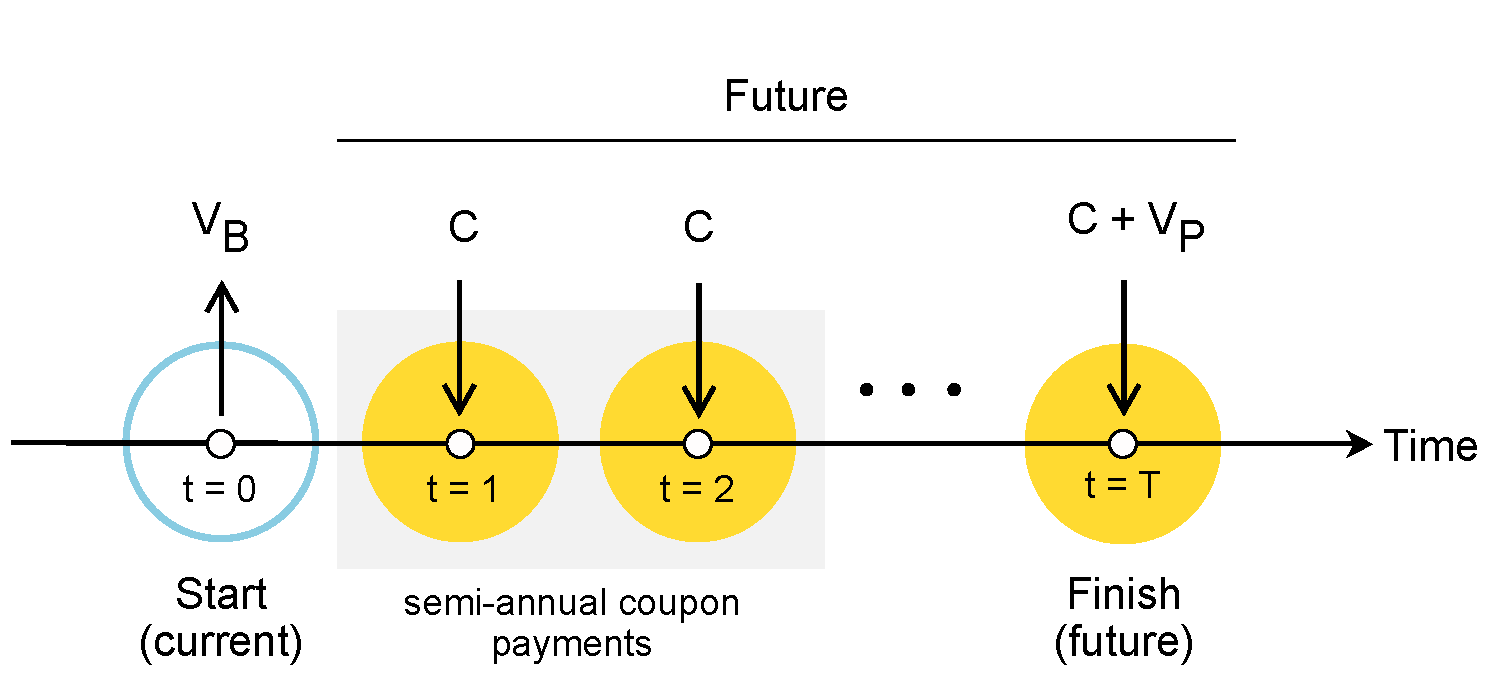
\includegraphics[width=0.85\textwidth]{./figs/Fig-Bond-Asset-Timeline-Schematic.pdf}
    \caption{Asbtract asset schematic of a coupon-bearing Treasury Note (T-note) or Bond (T-bond). 
	The lender (you) gives the United States Treasury 
    the price $V_{B}$ of the note (bond) at auction. In return, the Treasury pays the note (bond) holder (you) the face (par) value of the note (bond) $V_{P}$ at maturity. 
	The schematic is written from the note (bond) holder's perspective.}\label{fig:govt-note-bond-schematic}
\end{figure}
\href{https://treasurydirect.gov/marketable-securities/treasury-notes/}{United States Treasury Notes or T-notes}, 
are debt instruments that provide a stable interest payment every six months until maturity, called a coupon payment, and the face (par) value of the note at maturity (Fig. \ref{fig:govt-note-bond-schematic}).
Treasury notes are offered in terms of T = 2, 3, 5, 7, and 10 years and can be bought for more or less than their face (par) value. 
Upon maturity, the lender receives the entire face (par) value of the note. 
On the other hand,  \href{https://treasurydirect.gov/marketable-securities/treasury-bonds/}{United States Treasury Bonds or T-bonds} 
are coupon debt instruments with a maturity of more than 10 years, e.g., 20 or 30 years. S
imilar to notes, bonds are bought for more or less than their face (par) value and pay interest every six months until maturity.
The coupon rate (interest rate) and the yeild (discount factor) for these securities is fixed at issuance time, and remains constant over the lifetime of the security.
At maturity, the lender receives the bond's par value (or note) and a final coupon payment. 
Similar, to Tteasury bills, the pricing of notes and bonds is based on the present value of the future cash flows. 

\section*{The Pricing of Coupon-Bearing Treasury Securities}
We will use the abstract asset framework to develop a mathematical model for the price of coupon-bearing Treasury securities.
A \texttt{T}-year Treasury note (bond) with face value $V_{P}$, an effective yield $\bar{r}$, and $\lambda$ coupon payments per year, costs $V_{B}$ at auction.
The note (bond) price is the sum of discounted future coupon payments and face value, making the net present value (NPV) zero:
\begin{equation}
\text{NPV}(T,\bar{r}) = -V_{B} + \mathcal{D}^{-1}_{\lambda{T},0}(\bar{r})\cdot{V_{P}}+C\cdot\sum_{j=1}^{\lambda{T}}\mathcal{D}_{j,0}^{-1}(\bar{r}) = 0
\end{equation}
or equivalently:
\begin{equation}
V_{B} = \mathcal{D}^{-1}_{\lambda{T},0}(\bar{r})\cdot{V_{P}}+C\cdot\sum_{j=1}^{\lambda{T}}\mathcal{D}_{j,0}^{-1}(\bar{r})
\end{equation}
The term $\mathcal{D}_{j,0}^{-1}(\bar{r})$ represents the inverse multistep discount factor for period $0\rightarrow{j}$. 
The term $C\equiv(\bar{c}/\lambda)\cdot{V_{P}}$ represents the coupon payment, where $\bar{c}$ is the coupon rate.
Typically, the coupon rate is quoted as an annual rate, so we divide by $\lambda$ to get the semi-annual coupon payment.
Furher, Treasury notes and bonds typically pay coupons every six months, so $\lambda=2$.
Finally, the discounting for Treasury instruments uses a discrete compounding model, so the discount factor for these calculations takes the form:
\begin{equation}
\mathcal{D}_{j,0}(\bar{r}) = \left(1+\frac{\bar{r}}{\lambda}\right)^{j}
\end{equation}
where $j$ denotes the period number, and $\bar{r}$ is the effective yield (constant).


\clearpage
\printindex

\end{document}
